\nonstopmode

\documentclass[letterpaper,11pt,titlepage]{article}
\usepackage{amsthm,amssymb,mathtools}
\mathtoolsset{showonlyrefs}
\usepackage{bm}
\usepackage[margin=1in]{geometry}
\usepackage{booktabs}
\usepackage{enumitem}
\usepackage{framed}
\usepackage{tikz}
\usetikzlibrary{shapes,arrows.meta,positioning,patterns,calc}
\usepackage{pgfplots}
\pgfplotsset{compat=1.9}
\usepackage{listings}
%\usepackage[numbered,framed]{mcode}

\usepackage{algpseudocode}
\usepackage{algorithm}

\usepackage{fancyhdr}
\pagestyle{fancy}
\fancyhead{}
\fancyfoot{}
\fancyfoot[L]{K.\ Okkelberg}
\fancyfoot[R]{\thepage}
\renewcommand{\headrulewidth}{0pt}
\renewcommand{\footrulewidth}{0.5pt}

\newcommand*\dif{\mathop{}\!\mathrm{d}}
\newcommand{\trans}{^\text{T}}
\newcommand{\herm}{^\text{H}}
\DeclareMathOperator{\E}{E}
\DeclareMathOperator{\trace}{trace}
\DeclareMathOperator{\sign}{sign}
\let\Pr\relax
\DeclareMathOperator{\Pr}{P}
\newcommand*\pder[2]{\frac{\partial #1}{\partial #2}}
\newcommand*\R{\mathbb{R}}

\tikzstyle{line} = [draw,>=latex]
\tikzstyle{dot} = [circle,fill=black,inner sep=0pt,minimum size=4pt]

\begin{document}

\title{ECE 6553: Homework \#4}
\author{Klaus Okkelberg}
\date{March 30, 2017}
\maketitle

\setlist{listparindent=\parindent}

\begin{enumerate}[leftmargin=0pt]

    \item The following table shows the Hamiltonian, the optimality condition for $u$, the costate equation, and the transversality condition for the two formulations. We can see that the are equivalent problems.

        \begin{tabular}{l@{\hspace{1cm}}l}
            \toprule
            $L=1$, $\Psi=0$ & $L=0$, $\Psi=T$ \\
            \midrule
            $H=1+\lambda\trans f$ & $H=\lambda\trans f$ \\
            $\displaystyle\pder{H}{u}=\lambda\trans\pder{f}{u}=0$ &
            $\displaystyle\pder{H}{u}=\lambda\trans\pder{f}{u}=0$ \\[2ex]
            $\displaystyle\dot\lambda=-\pder{H\trans}{x}=-\pder{f\trans}{x}\lambda$ &
            $\displaystyle\dot\lambda=-\pder{H\trans}{x}=-\pder{f\trans}{x}\lambda$ \\[2ex]
            $\displaystyle H+\pder{\Psi}{T}\bigg|_{t=T}=1+\lambda\trans f + 0\Big|_{t=T}$ &
            $\displaystyle H+\pder{\Psi}{T}\bigg|_{t=T}=\lambda\trans f + \pder{T}{T}\bigg|_{t=T}$ \\[2ex]
            $\qquad= 1+\lambda\trans f\Big|_{t=T}$ &
            $\qquad= 1+\lambda\trans f\Big|_{t=T}$ \\
            \bottomrule
        \end{tabular}

    \item We add an augmented state to represent the energy constraint:
        \begin{align}
            \min_{u,T} {} & \int_0^T\!\dif t \\
            \text{s.t. } &
            \begin{aligned}[t]
                \dot x &= u, & x(0) = 0, && x(T) &= x_T \\
                \dot{\hat x} &= u^2, & \hat x(0) = 0, && \hat x(T) &= E
            \end{aligned} \\
            H &= 1 + \lambda u + \widehat\lambda u^2
        \end{align}
        The costate equations are
        \begin{align}
            \dot\lambda &= -\pder{H}{x} = 0 \Rightarrow \lambda = c_1 \\
            \dot{\widehat\lambda} &= -\pder{H}{\hat x} = 0 \Rightarrow \widehat\lambda = c_2
        \end{align}
        The optimal control is given by
        \begin{align}
            \pder{H}{u} &= \lambda + 2\widehat\lambda u = c_1 + 2c_2 u = 0 \\
            u &= -\frac{c_1}{2c_2} = k,
        \end{align}
        where $k$ is a constant.

        Applying the boundary conditions,
        \begin{align}
            x(T) &= x(0) + \int_0^T \dot x\dif t = 0 + \int_0^T u\dif t = kT = x_T \\
            \hat x(T) &= \hat x(0) + \int_0^T \dot{\hat x}\dif t = 0 + \int_0^T u^2 \dif t = k^2 T = E
        \end{align}
        The quotient of the second equation and the first is
        \begin{align}
            \frac{k^2 T}{kT} &= k = \frac{E}{x_T} \\
            \Rightarrow & \boxed{u=\frac{E}{x_T}} \\
            T &= \frac{x_T}{k} = \frac{x_T}{E/x_T} \\
            \Rightarrow & \boxed{T = \frac{x_T^2}{E}}
        \end{align}

    \item 
        \begin{enumerate}
            \item The problem is
                \begin{align}
                    \min_{u,T} {} & \int_0^T \!\dif t \\
                    \text{s.t. } & \dot x_1 = x_2 \\
                                 & \dot x_2 = -x_1 + u \\
                                 & u(t)\in[-1,1] \quad \forall t\in[0,T]
                \end{align}
                The Hamiltonian is $H = 1 + \lambda\trans f = 1 + \lambda_1 x_2 + \lambda_2 (-x_1 + u)$. Then, the costate equations are
                \begin{align}
                    \dot\lambda_1 &= -\pder{H}{x_1} = \lambda_2 \\
                    \dot\lambda_2 &= -\pder{H}{x_2} = -\lambda_1
                \end{align}
                We check the proposed $\lambda$ to see whether they fit these equations:
                \begin{align}
                    \dot\lambda_1 &= \frac{\dif}{\dif t} \Big[ \alpha\cos(T-t) + \beta\sin(T-t) \Big] \\
                                  &= -\alpha\sin(T-t)\frac{\dif}{\dif t}(T-t) + \beta\cos(T-t)\frac{\dif}{\dif t}(T-t) \\
                                  &= \alpha\sin(T-t) - \beta\cos(T-t) \\
                                  &= \lambda_2(t) \\
                    \dot\lambda_2 &= \frac{\dif}{\dif t} \Big[ \alpha\sin(T-t) - \beta\cos(T-t) \Big] \\
                                  &= \alpha\cos(T-t)\frac{\dif}{\dif t}(T-t) + \beta\sin(T-t)\frac{\dif}{\dif t}(T-t) \\
                                  &= - \Big[ \alpha\cos(T-t) + \beta\sin(T-t) \Big] \\
                                  &= -\lambda_1(t)
                \end{align}
                They indeed fit the costate equations.

            \item Applying the transversality condition gives
                \begin{align}
                    0 &= H + \pder{\Psi}{T} \bigg|_{t=T} = 1 + \lambda_1 x_2 + \lambda_2 (-x_1 + u) \Big|_{t=T} \\
                      &= 1 + \lambda_2(T) u(T) \quad \text{(since $x(T)=0$)}
                \end{align}
                Note that PMP gives the optimal control as $u=-\sign(\lambda_2)$, so
                \begin{align}
                    0 &= 1 + \lambda_2(T) \cdot -\sign(\lambda_2(T)) \\
                      &= 1 - \big| \lambda_2(T) \big| \\
                      &= 1 - \big| \alpha\sin 0 - \beta\cos 0 \big| \\
                    |\beta| &= 1 \\
                    \beta &= \pm 1
                \end{align}
                Additionally, this is a conservative system so $H$ is constant. Then,
                \begin{align}
                    0 &= H + \pder{\Psi}{T} \bigg|_{t=0} = 1 + \lambda_1 x_2 + \lambda_2 (-x_1 + u) \Big|_{t=0} \\
                      &= 1 + \lambda_1(0) x_2(0) - \lambda_2(0) x_1(0) - \big|\lambda_2(0)\big| \\
                      &= 1 + \big[\alpha\cos T + \beta\sin T\big] x_2(0) - \big[\alpha\sin T - \beta\cos T\big] x_1(0) - \big|\alpha\sin T - \beta\cos T\big| \\
                      &= 1 + \big[\alpha\cos T + \beta\sin T\big] x_2(0) - \big[\alpha\sin T - \beta\cos T\big] x_1(0) - \sqrt{\alpha^2 + \beta^2} \\
                      &= 1 + \big[\alpha\cos T \pm \sin T\big] x_2(0) - \big[\alpha\sin T \mp \cos T\big] x_1(0) - \sqrt{\alpha^2 + 1} \\
                    \alpha^2 + 1 &= \Big( 1 + \big[\alpha\cos T \pm \sin T\big] x_2(0) - \big[\alpha\sin T \mp \cos T\big] x_1(0) \Big)^2
                \end{align}
                This is quadratic in $\alpha$, so $\alpha$ can take on four values dependent on $x(0)$ and $T$ (and the sign of $\beta$), not necessary unique or real. For a given $x(0)$, the optimal values for $\alpha$ and $\beta$ are the real values that result in minimum $T$. 
        \end{enumerate}

    \item On a time interval of length $\pi$, sine and cosine switch sign at most once. (Zero sign switches happen if they are zero at $k\pi$). Additionally, using the angle sum identity
        \begin{gather}
            \sin(A + B) = \sin(A)\cos(B) + \cos(A)\sin(B),
        \end{gather}
        we can rewrite the costate equation as a single sinusoid:
        \begin{gather}
            \lambda_2(t) = \sqrt{\alpha^2+\beta^2} \sin(T-t + \phi), \quad \phi = \arctan \left(\frac{-\beta}{\alpha}\right).
        \end{gather}
        Therefore, $\lambda_2(t)$ switches sign at most once on that interval and the optimal control
        \begin{gather}
            u = -\sign(\lambda_2)
        \end{gather}
        also switches at most once (from $\pm 1$ to $\mp 1$).

        \clearpage
    \item The dynamics of the system are
        \begin{align}
            \dot x_1 &= x_2 \\
            \dot x_2 &= -x_1 + u
        \end{align}
        With $u=0$, this describes clockwise movement along a circle centered at the origin. Thus, with the control $u=\pm 1$, the circles are centered at $(\pm1,0)$.

        \begin{center}
            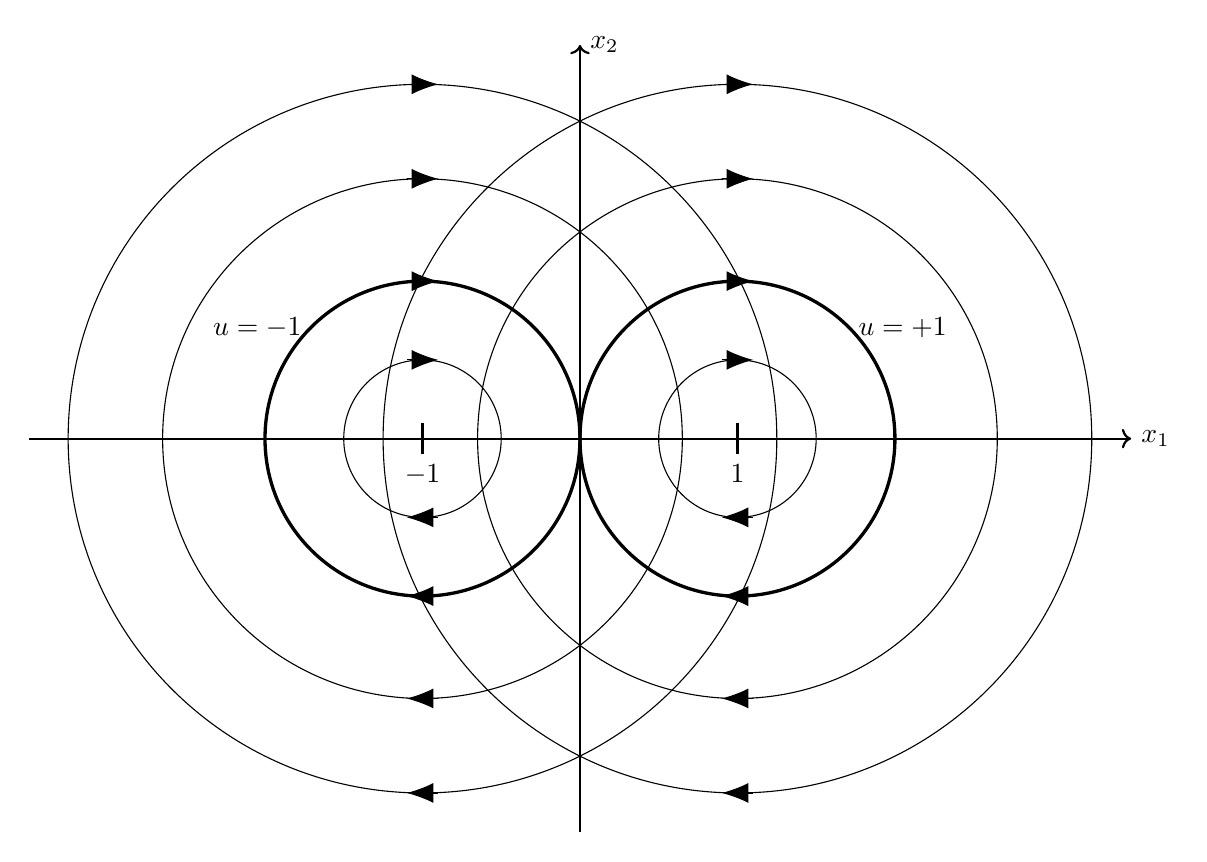
\begin{tikzpicture}
                \draw [thick,->] (-7,0) -- (7,0) node [right] {$x_1$};
                \draw [thick,->] (0,-5) -- (0,5) node [right] {$x_2$};
                \draw [thick] (2,0.2) -- (2,-0.2) node [below] {$1$};
                \draw [thick] (-2,0.2) -- (-2,-0.2) node [below] {$-1$};

                \foreach \r in {1,2,3.3,4.5,...,5}
                \foreach \u in {2,-2}
                {
                    \draw (\u,0) circle (\r);
                    \draw [-{Latex[scale=2]}] (\u-0.2,\r) -- (\u+0.2,\r);
                    \draw [{Latex[scale=2]}-] (\u-0.2,-\r) -- (\u+0.2,-\r);
                }

                \foreach \r in {2}
                \foreach \u in {2,-2}
                {
                    \draw [very thick] (\u,0) circle (\r);
                }

                \node [right] at ($(2,0)+(45:2)$) {$u=+1$};
                \node [left] at ($(-2,0)+(135:2)$) {$u=-1$};
                
                %\node at (6,4) {$u=+1$};
                %\node at (-6,4) {$u=-1$};
            \end{tikzpicture}
        \end{center}
        Note that each orbit takes the same amount of time to move around. The controller switches sign every $\pi$ seconds to get to an orbit whose radius is closer to 1 (closer to the orbits that reach the origin).

    \item Since the constraint is $y=Cx=0$ $\forall t$, then all derivatives of $y$ are also zero, i.e.
        \begin{align}
            0 &= y = Cx \\
            0 &= \dot y = C\dot x = C(Ax + Bu) = CAx + CBu \\
            0 &= \ddot y = CA \dot x + CB\dot u = CA^2 x + CABu + CB\dot u \\
            0 &= y^{(3)} = CA^2 \dot x + CAB\dot u + CB\ddot u = CA^3 x + CA^2Bu + CAB\dot u + CB\ddot u \\
              & \shortvdotswithin{=}
            0 &= y^{(d)} = CA^d x + CA^{d-1}Bu + \smash{\sum_{k=0}^{d-2}} \, CA^kB u^{(d-1-k)}
        \end{align}
        Since this system has relative degree $d$, $CA^kB=0$ for $k<d-1$, so
        \begin{align}
            0 &= CA^d x + CA^{d-1}B u \\
            u &= -(CA^{d-1}B)^{-1} CA^d x
        \end{align}
        Note that the optimal control only depends on the state.

        The optimality conditions of the system are
        \begin{gather}
            \boxed{
            \begin{aligned}
                H &= L + \lambda\trans f = x\trans Q x + u\trans R u + \lambda\trans(Ax + Bu) \\
                u &= -(CA^{d-1}B)^{-1} CA^d x \\
                \dot\lambda &= -\pder{H\trans}{x} = -2Qx - A\trans\lambda \\
                Cx_0 &= 0
            \end{aligned}
            }
        \end{gather}
        The optimal control and the costate are related by
        \begin{align}
            \pder{H}{u} &= 2u\trans R + \lambda\trans B = 0 \\
            u &= \frac{1}{2} R^{-1} B\trans \lambda
        \end{align}

\end{enumerate}

\end{document}
